%%%%%%%%%%%%%%%%%%%%%%%%%%%%%%%%%%%%%%%%%%%%%%%%%%
\section{Event Simulation}
%%%%%%%%%%%%%%%%%%%%%%%%%%%%%%%%%%%%%%%%%%%%%%%%%%
\subsection{Geant3, recombination, drift velocity}

We use GEANT3 for simulating energy deposition of beam particles and
their daughters. Readout pitch is 1 cm, 

we set the maximum step of Geant to 0.5 mm
which is enough smaller than the readout pitch of 1 cm.

It means charge deposition in one strip is typically 
simulated with 20 GEANT steps.

We set energy cut-off for soft electron/photon emission to
10 keV which is minimum possible energy can be set in GEANT3.
This cut-off is very important for  ionization electron recombination.

Recombination of electron and Argon ion depends on
the electric field and $dE/dx$. We use a measurement in Ref.\cite{658352}.
\begin{equation}
Q = A \frac{Q_0}{1 + k dE/dx}, A = 0.800, k = 0.486
\end{equation}

Velocity of the drift electron depends on the liquid Argon temperature
and the electric field. We use a measurement in Ref \cite{649233}.


\begin{verbatim}
 *     Special TPAR for TMED   3   Liquid_argon                                                    *
 *  CUTGAM= 10.00 keV  CUTELE= 10.00 keV  CUTNEU= 10.00 MeV  CUTHAD= 10.00 MeV  CUTMUO= 10.00 MeV  *
 *  BCUTE = 10.00 keV  BCUTM = 10.00 keV  DCUTE = 10.00 keV  DCUTM = 10.00 keV  PPCUTM= 10.00 MeV  *
 *  IPAIR=  1.  ICOMP=  1.  IPHOT=  1.  IPFIS=  0.  IDRAY=  1.  IANNI=  1.  IBREM=  1.  IHADR=  4. *
 *  IMUNU=  1.  IDCAY=  1.  ILOSS=  1.  IMULS=  1.  IRAYL=  0.  ILABS=  0.  ISYNC=  0.  ISTRA=  0. *
\end{verbatim}



\begin{itemize}
\item Plot: Geant Geometry, typical track (Tanaka)
\item Plot: recombination factor, drift velocity  (Tanaka)
\end{itemize}

\subsection{Electric Field}

Electric field of the TPC field cage
We have calculated the electric field using a 2D FEM (Finite Element Method) package \cite{Ref:FEMTET}.

This field map is used for simulating electron drift.


\begin{itemize}
\item Plot: 2D field map  (Tanaka)
\end{itemize}

\subsection{Drift Electron Diffusion}
\begin{itemize}
\item Plot: drift simulation  (Tanaka)
\end{itemize}

\subsection{Preamp Gain Calibration}
\begin{itemize}
\item Preamp gain vs channel number  (Naito)
\end{itemize}

%\subsection{FFT Noise}
\subsection{FFT Noise}
There are two kinds of noise in the data we obtained, random noise and coherent noise.
Random noise is the noise which exists in each anode channel.
Coherent noise is in each board.
The pseudo noise we implemented in Monte Carlo simulation is composed of random and coherent noise by this reason.

Random noise is generated from FFT(Fast Fourier Transform) distribution of real data. Figure \ref{example10ch} shows an example of FFT distribution.

Coherent noise is generated board by board as the noise scale in the real data we obtained.
The noise scale is defined as a root mean square of pedestal, minimum noise scale is about 3 and maximum noise scale is about 10 in the data.

The ratio of random and coherent noise is 1:1 as equation \ref{PseudoNoise}.
Figure \ref{DATAnoise} shows real data noise and Fig.\ref{MCnoise} shows pseudo noise we implemented in Monte Carlo simulation.
\begin{equation}
  Pseudo\,Noise = \frac{Random\,Noise + Coherent\,Noise}{2}
  \label{PseudoNoise}
\end{equation}

\begin{figure}[!htb]
  \centering
  \centering
  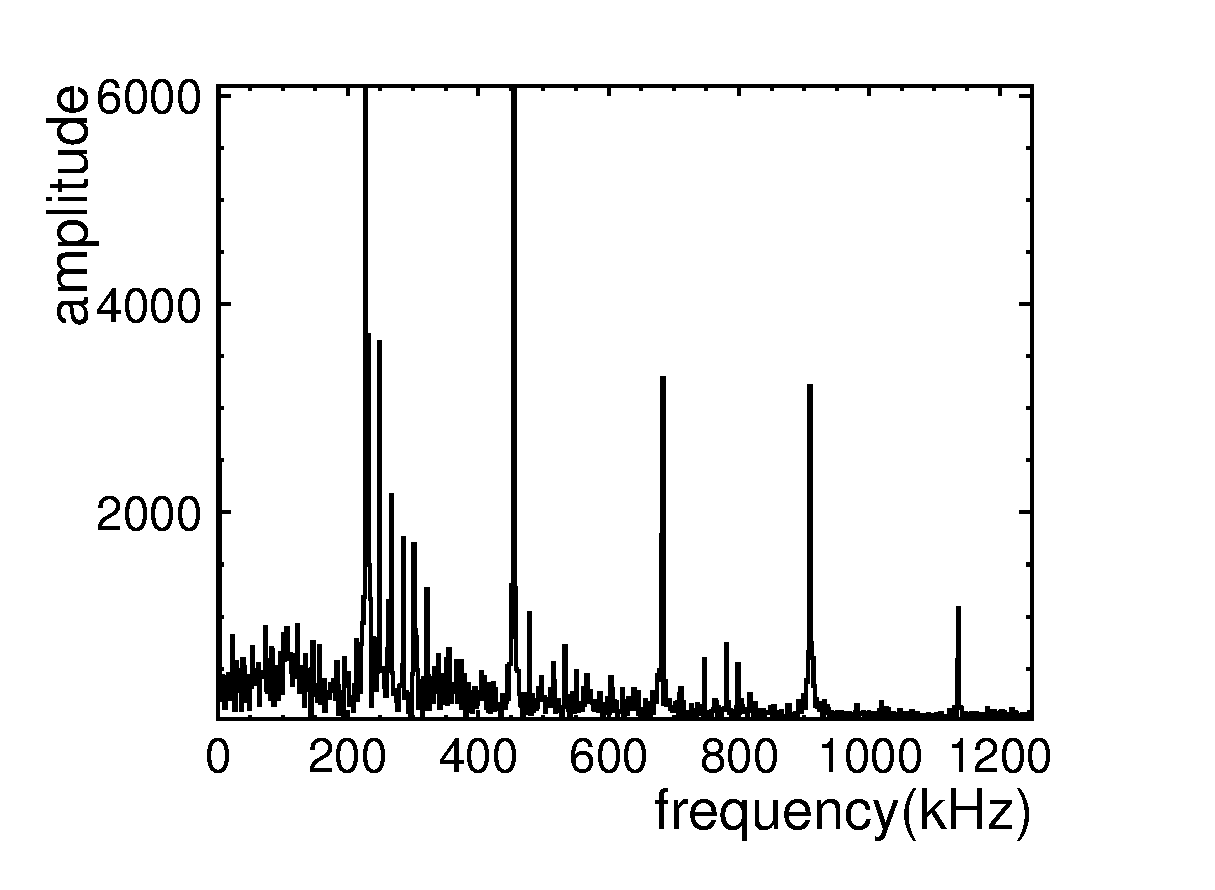
\includegraphics[width=10cm,clip]{./fig/FFTdist.eps}
  \caption{An example distribution of frequency}
  \label{example10ch}
\end{figure}
%\begin{figure}[!htb]
%  \centering
%  \centering
%  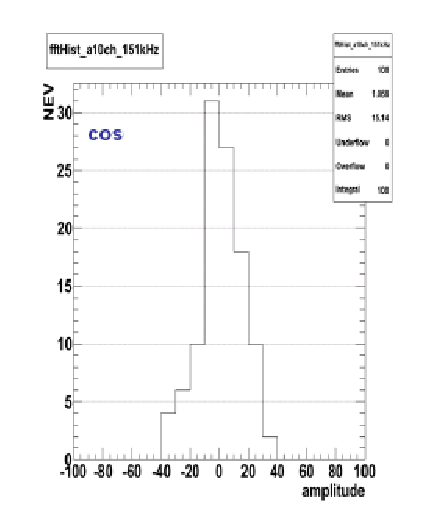
\includegraphics[width=11cm,clip]{./fig/cos.eps}
%  \caption{An example of distribution of amplitude}
%  \label{ampDist}
%\end{figure}
%\begin{figure}[!htb]
%  \centering
%  \centering
%  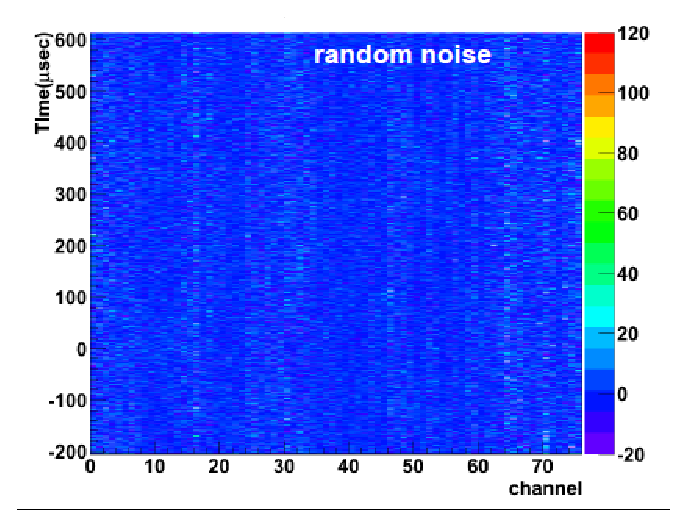
\includegraphics[width=11cm,clip]{./fig/randomnoise.eps}
%  \caption{Random noise}
%  \label{randomNoise}
%\end{figure}
\begin{figure}[!htb]
\begin{minipage}{0.5\hsize}
  \centering
  \includegraphics[width=7cm,clip]{./fig/DATAnoise.eps}
  \caption{Data noise}
  \label{DATAnoise}
\end{minipage}
\begin{minipage}{0.5\hsize}
  \centering
  \includegraphics[width=7cm,clip]{./fig/MCnoise.eps}
  \caption{Pseudo noise(Noise simulation)}
  \label{MCnoise}
\end{minipage}
\end{figure}
%\begin{figure}[!htb]
%  \centering
%  \centering
%  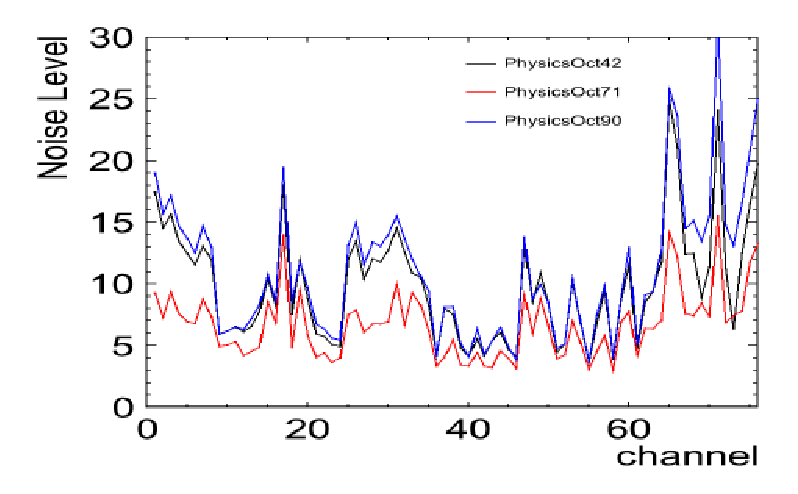
\includegraphics[width=11cm,clip]{./fig/scaling.eps}
%  \caption{Noise level}
%  \label{scaling}
%\end{figure}
\begin{itemize}
\item Plot: simulated event  (Nagasaka)
\end{itemize}

\subsection{Cross Talk}
\begin{itemize}
\item Plot: signal waveform (proton stopped point + 1)  (A. Okamoto)
\item Plot: simulated event with and without cross talk (A. Okamoto)
\end{itemize}

\subsection{Signal and Noise Scale Tuning}
\begin{itemize}
\item Plot: Landau distribution after the tuning  (Tanaka)
\end{itemize}

